\documentclass{report}
\usepackage[utf8]{inputenc} %encodage entrée
\usepackage{endnotes} %notes de fin
\usepackage{graphicx} %images
\usepackage[usenames,dvipsnames]{color} %couleurs
\usepackage{listings} %mise en forme de code source
\usepackage{xfrac}
\renewcommand\theequation{\arabic{equation}}
\usepackage{tabularx} % modifier la taille des cellules des tableaux
\usepackage{upquote}
\usepackage{textcomp}
\usepackage{pdfpages}
\usepackage[frenchb]{babel} %langue
\usepackage{amsmath} %affichage des matrices
\usepackage{lipsum} %génération de lipsum
\usepackage{verbatim} %code source
\usepackage{moreverb} %amélioration du package verbatim
\usepackage{titlesec} %formatage des chapitres
\titleformat{\chapter}[hang]{\bf\huge}{\thechapter}{2pc}{}
\usepackage[a4paper]{geometry} %mise en page
% \usepackage{varioref,amssymb,float} % polices 
% \usepackage{pgf,tikz} % permet de créer comme pstricks des figures en code LateX 
% \usetikzlibrary{calc} 
% \usepackage{pgflibraryarrows} % librairie liée à tikz 
% \usepackage{pgflibrarysnakes} 
% \usepackage{xcolor} % module de couleur pour tikz 
\geometry{hscale=0.8,vscale=0.8,centering}
%\lstinputlisting[language=Python, firstline=37, lastline=45]{source_filename.py}
\title{Algorithmes numériques -- Rapport \\ \vspace{0.5cm}Interpolation et Approximation}
\author{Axel Delsol, Pierre-Loup Pissavy}
\date{Décembre 2013}
\lstset{literate=
   {á}{{\'a}}1 {é}{{\'e}}1 {í}{{\'i}}1 {ó}{{\'o}}1 {ú}{{\'u}}1
   {Á}{{\'A}}1 {É}{{\'E}}1 {Í}{{\'I}}1 {Ó}{{\'O}}1 {Ú}{{\'U}}1
   {à}{{\`a}}1 {è}{{\`e}}1 {ì}{{\`i}}1 {ò}{{\`o}}1 {ò}{{\`u}}1
   {À}{{\`A}}1 {È}{{\`E}}1 {Ì}{{\`I}}1 {Ò}{{\`O}}1 {Ò}{{\`U}}1
   {ä}{{\"a}}1 {ë}{{\"e}}1 {ï}{{\"i}}1 {ö}{{\"o}}1 {ü}{{\"u}}1
   {Ä}{{\"A}}1 {Ë}{{\"E}}1 {Ï}{{\"I}}1 {Ö}{{\"O}}1 {Ü}{{\"U}}1
   {â}{{\^a}}1 {ê}{{\^e}}1 {î}{{\^i}}1 {ô}{{\^o}}1 {û}{{\^u}}1
   {Â}{{\^A}}1 {Ê}{{\^E}}1 {Î}{{\^I}}1 {Ô}{{\^O}}1 {Û}{{\^U}}1
   {œ}{{\oe}}1 {Œ}{{\OE}}1 {æ}{{\ae}}1 {Æ}{{\AE}}1 {ß}{{\ss}}1
   {ç}{{\c c}}1 {Ç}{{\c C}}1 {ø}{{\o}}1 {å}{{\r a}}1 {Å}{{\r A}}1
   {€}{{\EUR}}1 {£}{{\pounds}}1
}
\lstdefinestyle{customc}{
   belowcaptionskip=1\baselineskip,
   breaklines=true,
   otherkeywords={polynome},
   frame=L,
   xleftmargin=\parindent,
   language=C,
   showstringspaces=false,
   basicstyle=\footnotesize\ttfamily,
   keywordstyle=\bfseries\color{ForestGreen},
   commentstyle=\itshape\color{Plum},
   identifierstyle=\color{NavyBlue},
   stringstyle=\color{Orange},
   numbers=left,
   caption=Code : \lstname,
   captionpos=b,
}
\lstset{
upquote=true,
columns=flexible,
basicstyle=\ttfamily,
}
\addto\captionsfrench{\renewcommand{\figurename}{\textsc{Graphique}}}
\addto\captionsfrench{\renewcommand{\tablename}{\textsc{Tableau}}}
\renewcommand{\thefigure}{\thesection.\arabic{figure}}
\renewcommand{\thetable}{\thesection.\arabic{table}}
\renewcommand{\lstlistingname}{\textsc{Figure}}
\lstdefinestyle{apercu}{
  xleftmargin=2cm,
  xrightmargin=2cm,
  frame=single,
  breaklines=true,
  breakatwhitespace=true,
  breakindent=5pt,
  postbreak=\space,
  captionpos=b,
  escapeinside={\%*}{*)},
  showstringspaces=false,
  caption=Apercu : \lstname,
}
\begin{document}
  \maketitle
  \tableofcontents

  \chapter{Préambule}
    \section{Structure du programme}
      Nous avons conçu un programme principal avec menus, présenté sous la forme suivante :
      \begin{lstlisting}[style=apercu, name=Menu Principal]
Menu principal : Interpolation et Approximation

Entrez n le nombre de points : 
%*\textit{(Saisie de la série de points...)}*)

%*\textit{(Affichage du tableau correspondant...)}*)
Quelle résolution utiliser ?
1- Newton
2- Neuville
3- Régression Linéaire
4- Approximation par une fonction exponentielle
5- Approximation par une fonction "puissance"
9- Nouvelle série de points (Menu principal)
0- Quitter
Votre choix :
      \end{lstlisting}
      
      Au lancement, le programme demande la saisie des valeurs, qu'il stocke dans un tableau, puis affiche le menu. Après chaque résolution, il est possible de réutiliser le jeu de données (chaque méthode qui doit modifier les valeurs utilise un duplicata). \\
      
      Le menu principal est codé dans le fichier source \verb"main.c". Les méthodes sont codées dans des fichiers individuels à l'exception des méthodes d'approximation qui sont toutes codées dans le même fichier puisqu'elles présentent de nombreuses similarités. Les prototypes des fonctions sont écrits dans les headers correspondants. Enfin, un fichier source présenté en annexe page \pageref{fonctionspolynome} regroupe toutes les fonctions de manipulation de polynômes.\\
      La liste de tous ces fichiers est présentée figure \ref{arborescence}.\\
      
      Le stockage des valeurs se fait en double précision (type \verb"double", 64 bits) afin d'obtenir des résultats suffisamment précis pour tracer les courbes.\\
      Et nos fonctions utilisent une structure de polynôme (composée du degré et des coefficients), présentée figure \ref{structpoly}, pour faciliter la compréhension du code.\\
      
      \lstinputlisting[style=customc, name=Structure de Polynôme, label=structpoly, firstline=4, lastline=8, firstnumber=4]{polynome.h}
      \newpage
      \textbf{Note :} Pour des raisons de lisibilité, les polynômes résultats sont arrondis dans ce rapport. En revanche, les graphiques sont tracés avec les valeurs calculées par la machine (précision maximale possible pour le type de données).\\
      Les écarts donnés sont calculés par la machine juste après la résolution (on calcule la distance moyenne entre les points et la courbe).\\
      Les arrondis affichés dans le rapport sont retournés à la demande par le programme, au format \LaTeX, dans un fichier intitulé \verb"resultat".
      
      \lstinputlisting[style=apercu, name=Arborescence des fichiers \lstinline"C" et \lstinline"makefile", label=arborescence]{arborescence}
      
    \section{Compilation et Logiciels utilisés}
      \noindent La compilation est gérée par un \verb"makefile".\\
      Le compilateur utilisé est \verb"GCC".
      Il suffit de taper \verb"make" pour lancer la compilation, puis \verb"./main" pour lancer le programme.\\
      Pour nettoyer les fichiers temporaires, il faudra taper \verb"make clean".\\
      Ce \verb"makefile" permet également de générer ce rapport ainsi que quelques fichiers qui y sont intégrés.\\ \\
      Les représentations graphiques sont générées avec \verb"Asymptote", générateur vectoriel de graphiques.\\
      Les polynômes résultats sont vérifiés avec \verb"GeoGebra", qui permet ensuite de générer une trame de fichier source pour \verb"Asymptote".
  \chapter{Interpolation}
    \noindent L'interpolation, en analyse numérique, est un ensemble de méthodes permettant d'obtenir une équation mathématique passant par tous les points d'une liste donnée.
    \newline
    Pour cette partie, les équations mathématiques recherchées sont des polynômes.
    \newline
    
    \underline{Notation pour la suite :}
    \vspace{0.1 cm}
    \begin{itemize}
      \item{La liste comporte $N$ éléments $(x_{i},y_{i})$.}
      \item{Les polynômes recherchés sont de la forme \[P_{N-1}(x)= \sum_{i=0}^{N-1} (a_{i} \cdot x^{i})\].}
    \end{itemize}
    \section{Méthode de Newton}
      \subsection{Présentation}
	\noindent La forme du polynôme par la méthode de Newton est la suivante : 
    	
    	\[P_{N-1}(x)= \sum_{i=0}^{N-1} \left( a_{i} \cdot \prod_{j=1}^{i} (x-x_{j}) \right)\] \\
	Pour ce faire, on utilise une méthode de recherche de coefficients récursive appelée méthode des \textit{différences divisées}. Le calcul des valeurs des différences divisées se fait à l'aide de fonctions : \\
    	
    	\noindent La différence divisée de degré $0$ est : $\forall i \in \{1, \cdots, N\}$, \indent $\nabla^{0}_{y_{i}} = y_{i}$.\\
    	 
	\noindent La différence divisée de degré $k$ est : $\forall i \in \{k+1,\cdots,N\}$, \indent $\nabla^{k}_{y_{i}} = \frac{\nabla^{k-1}_{y_{i}}-\nabla^{k-1}_{y_{k}}}{x_{i}-x_{k}}$.\\
    	 
    	\noindent Ensuite, on a directement les coefficients du polynôme de Newton par la relation\\
    	$ \forall i \in \{1, \cdots, N-1\}$, \indent $a_{i} = \nabla^{i}_{y_{(i+1)}}$.\\
    	 
    	\noindent Enfin, on peut retrouver la forme développée du polynôme à l'aide de la relation suivante :\\ \\
    	$\forall i \in \{0,\cdots,N\}$, \indent
    	$P_{i}(x) = \left\{
	\begin{array}{l l}
	  a_{N-1} & \quad \text{si $i$=0}\\
	  a_{N-1-i} + (x-x_{N-i}) \cdot P_{i-1}(x) & \quad \text{sinon}
	\end{array} \right. $. 
      \subsection{Programme}
	\lstinputlisting[style=customc]{newton.c}
    \newpage
    \section{Méthode de Neuville}
      \subsection{Présentation}
	Cette méthode permet d'exprimer le polynôme $P_{N-1}[x_{1},\cdots,x_{N}]$ sur les points $\{1,\cdots,N\}$ en fonction des polynômes $P_{N-2}[x_{1},\cdots,x_{N-1}]$ et $P_{N-2}[x_{2},\cdots,x_{N}]$ sur l'ensemble des points $\{1,\cdots,N-1\}$ et $\{2,\cdots,N\}$.\\
	
	\noindent L'expression est donnée sous la forme suivante : 
	
	$P_{k}[x_{i},\cdots,x_{i+k}](x) = \frac{(x-x_{i+k}) \cdot P_{k-1}[x_{i},\cdots,x_{i+k-1}](x) + (x_{i}-x) \cdot P_{k-1}[x_{i+1},\cdots,x_{i+k}](x)}{x_{i}-x{i+k}}, \forall x, \forall k=2,\cdots,N-1$ 
      \subsection{Programme}
	\lstinputlisting[style=customc]{neuville.c}
    \newpage
    \section{Résultats de tests}
      \subsection{Exemple tiré d'un TD}
	\begin{table}[h]
	  \centering
	  \begin{tabular}{| c | c | c | c | c |}
	  \hline 
	  $x_{i}$ & $1$ & $2$ & $3$ & $4$ \\ 
	  \hline 
	  $y_{i}$ & $0$ & $0$ & $0$ & $6$ \\ 
	  \hline 
	  \end{tabular}
	  \caption{Série 1}
	  \label{inter_td3_ex3}
	\end{table}
	
	\noindent\textbf{Méthode de Newton :}\\
	$P(x)= -6.00 + 11.00 \cdot x- 6.00 \cdot x^{2}  + 1.00 \cdot x^{3} $\\
	Erreur : $0$
	\newline
	
	\noindent\textbf{Méthode de Neuville :}\\
	$P(x)= -6.00 + 11.00 \cdot x- 6.00 \cdot x^{2}  + 1.00 \cdot x^{3} $\\
	Erreur : $0$
	\newline
	\newline
	
	\begin{figure}[h]
	  \centering
	  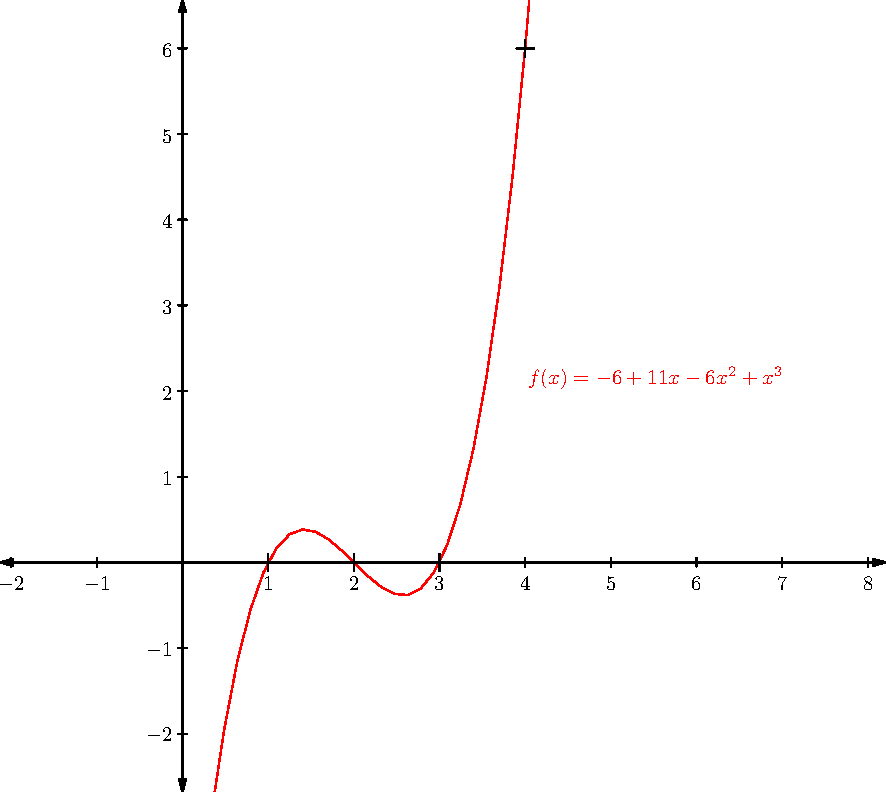
\includegraphics[scale=0.7]{graphiques/pdf_output/inter_test1.pdf}
	  \caption{Interpolations de Newton et Neuville -- (Tableau \ref{inter_td3_ex3})}
	\end{figure}
      \newpage
      
      \subsection{Densité de l'eau en fonction de la température}      
	\begin{table}[h]
	  \centering
	  \begin{tabular}{| c | c | c | c | c | c | c | c | c | c | c |}
	    \hline 
	    $x_{i}$ & $0$ & $2$ & $4$ & $6$ & $8$ & $10$ & $12$ & $14$ & $16$ & $18$ \\
	    \hline 
	    $y_{i}$ & $0.999870$ & $0.999970$ & $1.000000$ & $0.999970$ & $0.999880$ & $0.999730$ & $0.999530$ & $0.999530$ & $0.998970$ & $0.998460$ \\ 
	    \hline 
	  \end{tabular}
	  \begin{tabular}{| c | c | c | c | c | c | c | c | c | c | c |}
	    \hline
	    $x_{i}$ & $20$ & $22$ & $24$ & $26$ & $28$ & $30$ & $32$ & $34$ & $36$ & $38$ \\ 
	    \hline
	    $y_{i}$ & $0.998050$ & $0.999751$ & $0.997050$ & $0.996500$ & $0.996640$ & $0.995330$ & $0.994720$ & $0.994720$ & $0.993330$ & $0.993260$ \\
	    \hline
	  \end{tabular}
	  \caption{Mesures}
	  \label{inter_tp2_ex1_densite}
	\end{table}
	
	\noindent\textbf{Méthode de Newton :}\\
	$P(x) \approx 0.999870 + 7.693711 \cdot x - 13.276666 \cdot x^{2}  + 9.932303 \cdot x^{3} - 4.345460 \cdot x^{4}  + 1.259124 \cdot x^{5} - 0.258585 \cdot x^{6}  + 0.039240 \cdot x^{7} - 0.004520 \cdot x^{8}  + 0.000402 \cdot x^{9} - 0.000028 \cdot x^{10}  + 0.000002 \cdot x^{11} - 0.000000 \cdot x^{12}  + 0.000000 \cdot x^{13} - 0.000000 \cdot x^{14}  + 0.000000 \cdot x^{15} - 0.000000 \cdot x^{16}  + 0.000000 \cdot x^{17} - 0.000000 \cdot x^{18}  + 0.000000 \cdot x^{19} $\\
	Erreur : $0.000002166566117323$
	\newline
	
	\noindent\textbf{Méthode de Neuville :}\\
	$P(x) \approx 0.999870 + 7.693711 \cdot x- 13.276666 \cdot x^{2}  + 9.932303 \cdot x^{3} - 4.345460 \cdot x^{4}  + 1.259124 \cdot x^{5} - 0.258585 \cdot x^{6}  + 0.039240 \cdot x^{7} - 0.004520 \cdot x^{8}  + 0.000402 \cdot x^{9} - 0.000028 \cdot x^{10}  + 0.000002 \cdot x^{11} - 0.000000 \cdot x^{12}  + 0.000000 \cdot x^{13} - 0.000000 \cdot x^{14}  + 0.000000 \cdot x^{15} - 0.000000 \cdot x^{16}  + 0.000000 \cdot x^{17} - 0.000000 \cdot x^{18}  + 0.000000 \cdot x^{19} $\\
	Erreur : $0.000028505775100296$
	\newline
	\newline
		  
	\begin{figure}[h]
	  \centering
	  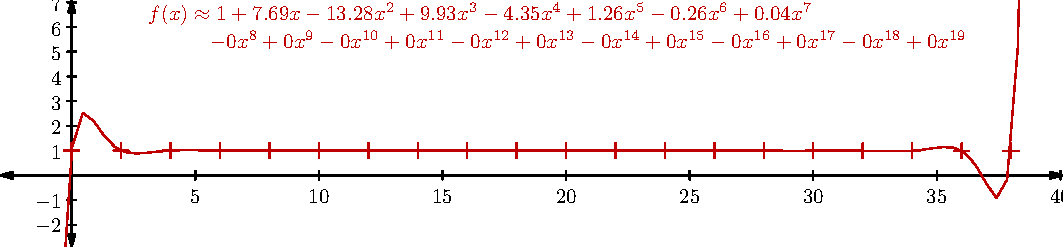
\includegraphics{graphiques/pdf_output/inter_tp2_ex1.pdf}
	  \caption{Interpolation de Newton et Neuville -- (Tableau \ref{inter_tp2_ex1_densite})}
	\end{figure}
      \newpage
    
      \subsection{3 séries}
	\begin{table}[h]
	  \centering
	  \begin{tabular}{| c | c | c | c | c | c | c | c | c | c | c | c |}
	    \hline 
	    $x_{i}$ & $10$ & $8$ & $13$ & $9$ & $11$ & $14$ & $6$ & $4$ & $12$ & $7$ & $5$ \\ 
	    \hline 
	    $y^{(1)}_{i}$ & $9.14$ & $8.14$ & $8.74$ & $8.77$ & $9.26$ & $8.10$ & $6.13$ & $3.10$ & $9.13$ & $7.26$ & $4.74$ \\ %s1
	    \hline 
	    $y^{(2)}_{i}$ & $7.46$ & $6.77$ & $12.74$ & $7.11$ & $7.81$ & $8.84$ & $6.08$ & $5.39$ & $8.15$ & $6.42$ & $5.73$ \\ %s2
	    \hline 
	    $y^{(3)}_{i}$ & $6.58$ & $5.76$ & $7.71$ & $8.84$ & $8.47$ & $7.04$ & $5.25$ & $12.50$ & $5.56$ & $7.91$ & $6.89$ \\ %s3 
	    \hline 
	  \end{tabular}	
	  \caption{Trois séries S1, S2, S3}
	  \label{inter_tp2_ex2_3series}
	\end{table}
	
	
	\noindent \underline{\textbf{Série 1 :}} \\ \\
	\textbf{Méthode de Newton :}\\
	$P(x) \approx -229.550000 + 299.165750 \cdot x- 173.107636 \cdot x^{2}  + 58.546955 \cdot x^{3} - 12.731862 \cdot x^{4}  + 1.859906 \cdot x^{5} - 0.184968 \cdot x^{6}  + 0.012375 \cdot x^{7} - 0.000533 \cdot x^{8}  + 0.000013 \cdot x^{9} - 0.000000 \cdot x^{10} $\\
	Erreur : $0.000000000016217532$
	\newline
	\newline
	\textbf{Méthode de Neuville :}\\
	$P(x) \approx -229.550000 + 299.165750 \cdot x- 173.107636 \cdot x^{2}  + 58.546955 \cdot x^{3} - 12.731862 \cdot x^{4}  + 1.859906 \cdot x^{5} - 0.184968 \cdot x^{6}  + 0.012375 \cdot x^{7} - 0.000533 \cdot x^{8}  + 0.000013 \cdot x^{9} - 0.000000 \cdot x^{10} $\\
	Erreur : $0.000000000012119518$
	\newline
	\newline
	
	\noindent\underline{\textbf{Série 2 :}} \\ \\
	\textbf{Méthode de Newton :}\\
	$P(x) \approx -12345.190000 + 16608.066492 \cdot x- 9870.941498 \cdot x^{2}  + 3416.593892 \cdot x^{3} - 763.094009 \cdot x^{4}  + 114.979985 \cdot x^{5} - 11.842442 \cdot x^{6}  + 0.823658 \cdot x^{7} - 0.037039 \cdot x^{8}  + 0.000973 \cdot x^{9} - 0.000011 \cdot x^{10} $\\
	Erreur : $0.000000000774325735$
	\newline
	\newline
	\textbf{Méthode de Neuville :}\\
	$P(x) \approx -12345.190000 + 16608.066492 \cdot x- 9870.941498 \cdot x^{2}  + 3416.593892 \cdot x^{3} - 763.094009 \cdot x^{4}  + 114.979985 \cdot x^{5} - 11.842442 \cdot x^{6}  + 0.823658 \cdot x^{7} - 0.037039 \cdot x^{8}  + 0.000973 \cdot x^{9} - 0.000011 \cdot x^{10} $\\
	Erreur : $0.000000001033081661$
	\newline
	\newline
	
	\noindent\underline{\textbf{Série 3 :}} \\ \\
	\textbf{Méthode de Newton :}\\
	$P(x) \approx -568559.640000 + 739678.381270 \cdot x- 424130.450858 \cdot x^{2}  + 141275.523224 \cdot x^{3} - 30298.693006 \cdot x^{4}  + 4375.222059 \cdot x^{5} - 431.155992 \cdot x^{6}  + 28.652640 \cdot x^{7} - 1.229803 \cdot x^{8}  + 0.030806 \cdot x^{9} - 0.000342 \cdot x^{10} $\\
	Erreur : $0.000000081067879843$
	\newline
	\newline
	\textbf{Méthode de Neuville :}\\
	$P(x) \approx -568559.640000 + 739678.381270 \cdot x- 424130.450858 \cdot x^{2}  + 141275.523224 \cdot x^{3} - 30298.693006 \cdot x^{4}  + 4375.222059 \cdot x^{5} - 431.155992 \cdot x^{6}  + 28.652640 \cdot x^{7} - 1.229803 \cdot x^{8}  + 0.030806 \cdot x^{9} - 0.000342 \cdot x^{10} $\\
	Erreur : $0.000000035876804073$
	\newpage
	\begin{figure}[h]
	  \centering
  	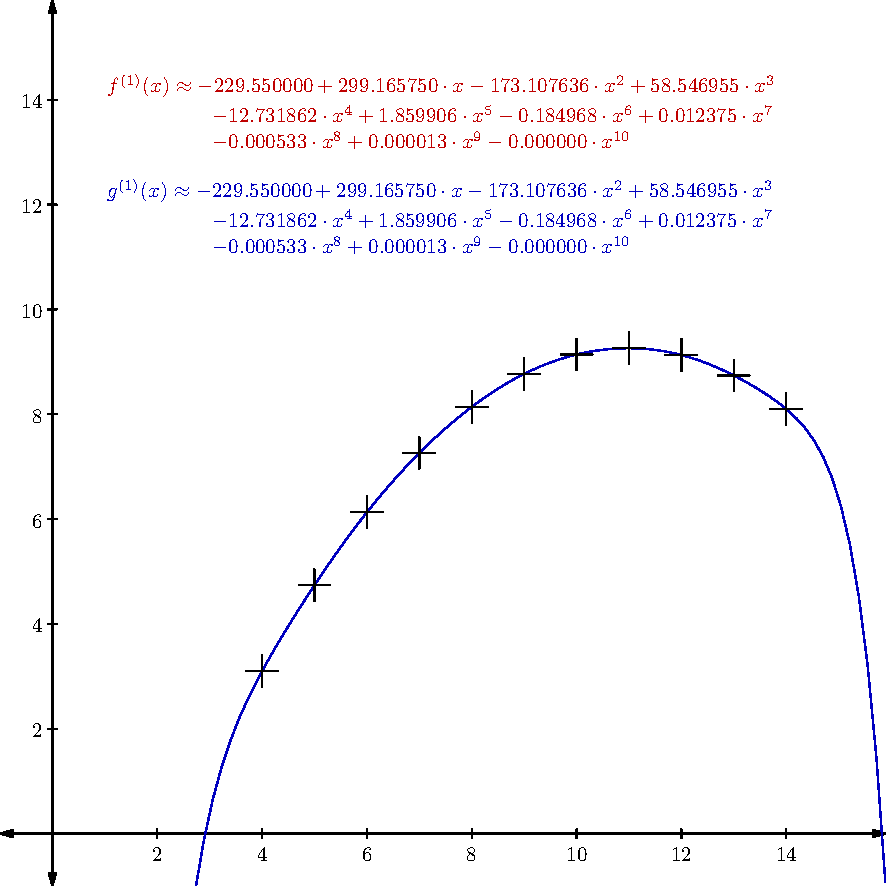
\includegraphics[scale=0.5]{graphiques/pdf_output/inter_tp2_ex2_1.pdf}
	  \caption{Interpolations de Newton et Neuville -- Série 1 (Tableau \ref{inter_tp2_ex2_3series})}
	\end{figure}
	\begin{figure}[h]
	  \centering
	  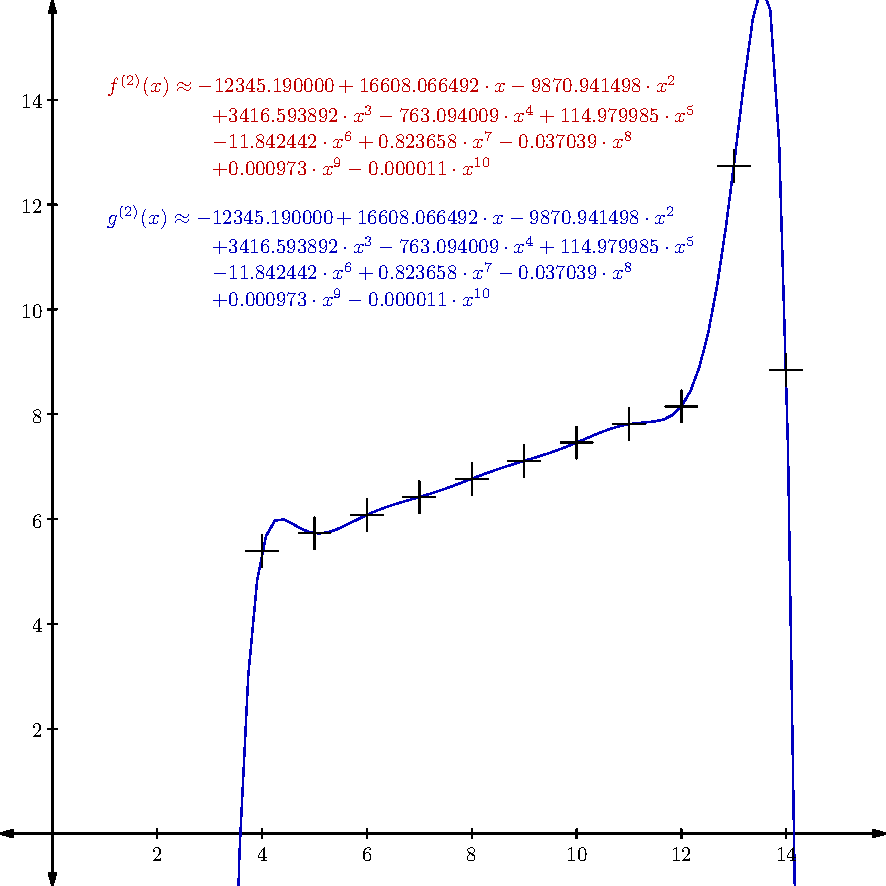
\includegraphics[scale=0.5]{graphiques/pdf_output/inter_tp2_ex2_2.pdf}
	  \caption{Interpolations de Newton et Neuville -- Série 2 (Tableau \ref{inter_tp2_ex2_3series})}
	\end{figure}
	\newpage
	\begin{figure}[h]
	  \centering
 	  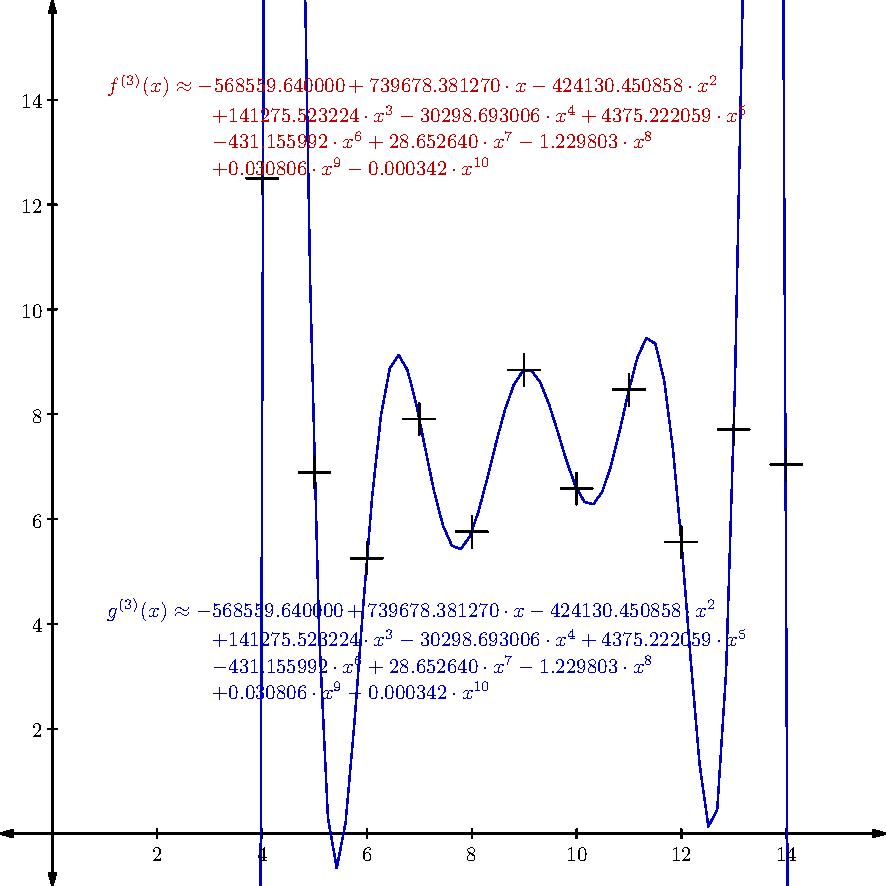
\includegraphics[scale=0.5]{graphiques/pdf_output/inter_tp2_ex2_3.pdf}
	  \caption{Interpolations de Newton et Neuville -- Série 3 (Tableau \ref{inter_tp2_ex2_3series})}
	\end{figure}
      \newpage
      \subsection{Dépenses et Revenus}
      \begin{table}[h]
% 	\centering
	\begin{tabular}{| c | c | c | c | c | c | c | c | c | c | c | c |}
	  \hline 
	  $x_{i}$ (R) & $752$ & $855$ & $871$ & $734$ & $610$ & $582$ & $921$ & $492$ & $569$ & $462$ & $907 $ \\ 
	  \hline 
	  $y_{i}$ (D) & $85$ & $83$ & $162$ & $79$ & $81$ & $83$ & $281$ & $81$ & $81$ & $80$ & $243 $ \\ 
	  \hline 
	\end{tabular}
	\newline
	\begin{tabular}{| c | c | c | c | c | c | c | c | c | c | c |}
	\hline 
	$x_{i}$ (R) & $643$ & $862$ & $524$ & $679$ & $902$ & $918$ & $828$ & $875$ & $809$ & $894$ \\ 
	\hline 
	$y_{i}$ (D) & $84$ & $84$ & $82$ & $80$ & $226$ & $260$ & $82$ & $186$ & $77$ & $223$ \\ 
	\hline 
	\end{tabular}
	\caption{Série non-triée}
	\label{inter_tp2_ex3_depenses}
      \end{table}
      
      \begin{table}[h]
	\centering
	\begin{tabular}{| c | c | c | c | c | c | c | c | c | c | c | c | c | c | c |}
	  \hline 
	  $x_{i}$ (R) & $752$ & $855$ & $828$ & $734$ & $809$ & $610$ & $582$ & $492$ & $569$ & $462$ & $643$ & $862$ & $524$ & $679$ \\ 
	  \hline 
	  $y_{i}$ (D) & $85$ & $83$ & $82$ & $79$ & $77$ & $81$ & $83$ & $81$ & $81$ & $80$ & $84$ & $84$ & $82$ & $80$ \\ 
	  \hline 
	\end{tabular}
	\caption{Série triée : Partie Basse}
	\label{inter_tp2_ex3_depenses_bas}
      \end{table}
      \begin{table}[h]
	\centering
	\begin{tabular}{| c | c | c | c | c | c | c | c |}
	  \hline 
	  $x_{i}$ (R) & $902$ & $918$ & $871$ & $875$ & $921$ & $907$ & $894$ \\ 
	  \hline 
	  $y_{i}$ (D) & $226$ & $260$ & $162$ & $186$ & $281$ & $243$ & $223$ \\ 
	  \hline 
	\end{tabular}
	\caption{Série triée : Partie Haute}
	\label{inter_tp2_ex3_depenses_haut}
      \end{table}
      
      
      \noindent\underline{\textbf{Partie Basse :}} \\ \\
      \textbf{Méthode de Newton :}\\
	$P(x) \approx 73581192209.962601-1459287367.863513 \cdot x + 13300351.970502 \cdot x^{2} - 73765.523297 \cdot x^{3}  + 277.759281 \cdot x^{4} - 0.749863 \cdot x^{5}  + 0.001493 \cdot x^{6} - 0.000002 \cdot x^{7}  + 0.000000 \cdot x^{8} - 0.000000 \cdot x^{9}  + 0.000000 \cdot x^{10} - 0.000000 \cdot x^{11}  + 0.000000 \cdot x^{12} - 0.000000 \cdot x^{13} $\\
	Erreur : $0.018460432587224723$
	\newline
	\newline
	\textbf{Méthode de Neuville :}\\
	$P(x) \approx 73581192209.952133-1459287367.863373 \cdot x + 13300351.970501 \cdot x^{2} - 73765.523297 \cdot x^{3}  + 277.759281 \cdot x^{4} - 0.749863 \cdot x^{5}  + 0.001493 \cdot x^{6} - 0.000002 \cdot x^{7}  + 0.000000 \cdot x^{8} - 0.000000 \cdot x^{9}  + 0.000000 \cdot x^{10} - 0.000000 \cdot x^{11}  + 0.000000 \cdot x^{12} - 0.000000 \cdot x^{13} $\\
	Erreur : $0.192499821369502971$
	\newline
	\newline
	
	\noindent\underline{\textbf{Partie Haute :}} \\ \\
	\textbf{Méthode de Newton :}\\
	$P(x) \approx 621022623331.547363-4157904770.816573 \cdot x + 11598209.746191 \cdot x^{2} - 17253.085748 \cdot x^{3}  + 14.435304 \cdot x^{4} - 0.006441 \cdot x^{5}  + 0.000001 \cdot x^{6} $\\
	Erreur : $0.000429349286215646$
	\newline
	\newline
	\textbf{Méthode de Neuville :}\\
	$P(x) \approx 621022623331.548340-4157904770.816572 \cdot x + 11598209.746191 \cdot x^{2} - 17253.085748 \cdot x^{3}  + 14.435304 \cdot x^{4} - 0.006441 \cdot x^{5}  + 0.000001 \cdot x^{6} $\\
	Erreur : $0.002443850040435791$
      \newpage
      \begin{figure}[h]
	\centering
	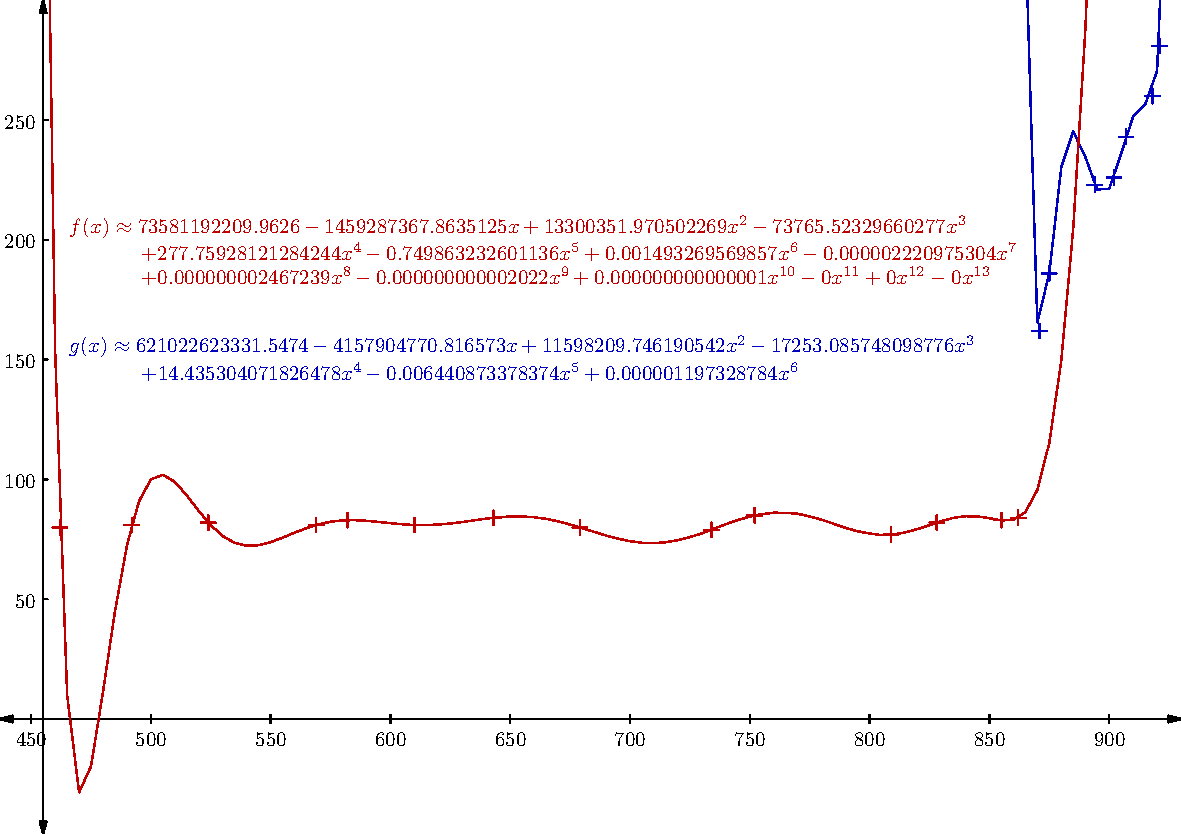
\includegraphics[scale=0.85]{graphiques/pdf_output/inter_tp2_ex3.pdf}
	\caption{Interpolation de Newton et Neuville -- (Tableaux \ref{inter_tp2_ex3_depenses_bas} \& \ref{inter_tp2_ex3_depenses_haut})}
      \end{figure}
    \newpage
    \section{Comparaison}
  \chapter{Approximation}
    Contrairement aux interpolations, les équations obtenues ne passent pas forcément par les $N$ points. On cherche uniquement à minimiser la distance moyenne entre les $N$ points mesurés et la courbe. Cette méthode est appelée \textit{méthode des moindres carrés}.\\
    Note : On n'aura donc pas à considérer une précision très importante pour comparer les tests, puisqu'il s'agit d'approximation, ce qui implique des écarts relativement importants.
    \section{Régression linéaire}
      \subsection{Présentation}
	La régression linéaire est un cas particulier de la méthode des moindres carrés. L'équation recherchée ici est une droite d'équation $y=a_{0} + a_{1} \cdot x$. On obtient alors le système :
	
	\begin{equation*}
	  \begin{bmatrix}
	    \overset{N}{\underset{i=1}{\sum}} x_{i}^{0} & \overset{N}{\underset{i=1}{\sum}} x_{i}^{1} \\
	    \overset{N}{\underset{i=1}{\sum}} x_{i}^{1} & \overset{N}{\underset{i=1}{\sum}} x_{i}^{2} \\
	  \end{bmatrix}
	  \cdot
	  \begin{bmatrix}
	    a_{0} \\
	    a_{1} \\
	  \end{bmatrix}
	  =
	  \begin{bmatrix}
	    \overset{N}{\underset{i=1}{\sum}} y_{i} x_{i}^{0} \\
	    \overset{N}{\underset{i=1}{\sum}} y_{i} x_{i}^{1} \\
	  \end{bmatrix}
	\end{equation*}
	
	On a enfin une expression pour $a_{0}$ et $a_{1}$ :
	
	\begin{displaymath}
	  a_{1} = \frac{\overline{yx}-\overline{x}\overline{y}}{\overline{x^{2}}-(\overline{x})^2}
	\end{displaymath}
	\vspace{0.1 cm}
	\begin{displaymath}
	  a_{0} = \overline{y} - a_{1} \cdot \overline{x}
	\end{displaymath}
      \subsection{Programme}
	\lstinputlisting[style=customc, lastline=79]{reglin.c}
    \newpage
    \section{Ajustement exponentiel}
      \subsection{Présentation}
	\noindent On doit trouver une équation sous la forme $y=c e^{dx}$.\\
	On a donc  $\ln (y)=\ln(c)+dx\ln(e)\Leftrightarrow \ln(y)=\ln(c)+dx$.\\
	Cela revient à effectuer une régression linéaire sous la forme :\\
	$Y=a_{0} + a_{1}x$ avec $Y=\ln(y)$, $a_{0}=\ln(c)$ et $a_{1}=d$.\\
	Finalement, on obtient $c=e^{a_0}$ et $d=a_1$.
      \subsection{Programme}
	\lstinputlisting[style=customc, firstline=80, lastline=120, firstnumber=80]{reglin.c}
    \newpage
    \section{Ajustement de type ``puissance"}
      \subsection{Présentation}
	\noindent On doit trouver une équation sous la forme $y=a x^{b}$.\\
	On a donc $\ln(y)=\ln(a) + b\ln(x)$.\\
	Cela revient à effectuer une régression linéaire sous la forme : \\
	$Y=a_{0} + a_{1}X$ avec $Y=\ln(y)$, $X=\ln(x)$, $a_{0}=\ln(a)$, et $a_{1}=b$.\\
	Finalement, on obtient $a=e^{a_0}$ et $b=a_1$.
      \subsection{Programme}
	\lstinputlisting[style=customc, firstline=122, firstnumber=122]{reglin.c}
    \newpage
    \section{Résultats de tests}
      \subsection{Exemple tiré d'un TD}
	\begin{table}[h]
	  \centering
	  \begin{tabular}{| c | c | c | c | c | c |}
	    \hline 
	    $x_{i}$ & $0.5$ & $1$ & $1.5$ & $2$ & $2.5$ \\ 
	    \hline 
	    $y_{i}$ & $0.49$ & $1.6$ & $3.36$ & $6.44$ & $10.16$ \\ 
	    \hline 
	  \end{tabular}
	  \caption{Exemple}
	  \label{approx_td3_ex6}
	\end{table}
	
	\noindent \textbf{Régression linéaire : } \\
	$P(x) = 4.836x - 2.844$\\
	Erreur : $0.732$
	\newline
	\newline
	\textbf{Ajustement par une fonction exponentielle :}\\
	$P(x) = 0.299115x \times e^{1.491228x}$\\
	Erreur : $0.758042$
	\newline
	\newline
	\textbf{Ajustement par une fonction ``puissance" :}\\
	$P(x) = 1.70314\times x^{1.88175}$\\
	Erreur : $0.23913$
	\newline
	
	On notera que pour ce jeu de points, c'est l'ajustement de type ``puissance" qui est le plus approprié puisque l'erreur est la plus faible parmi les trois méthodes.
	\begin{figure}[h]
	  \centering
	  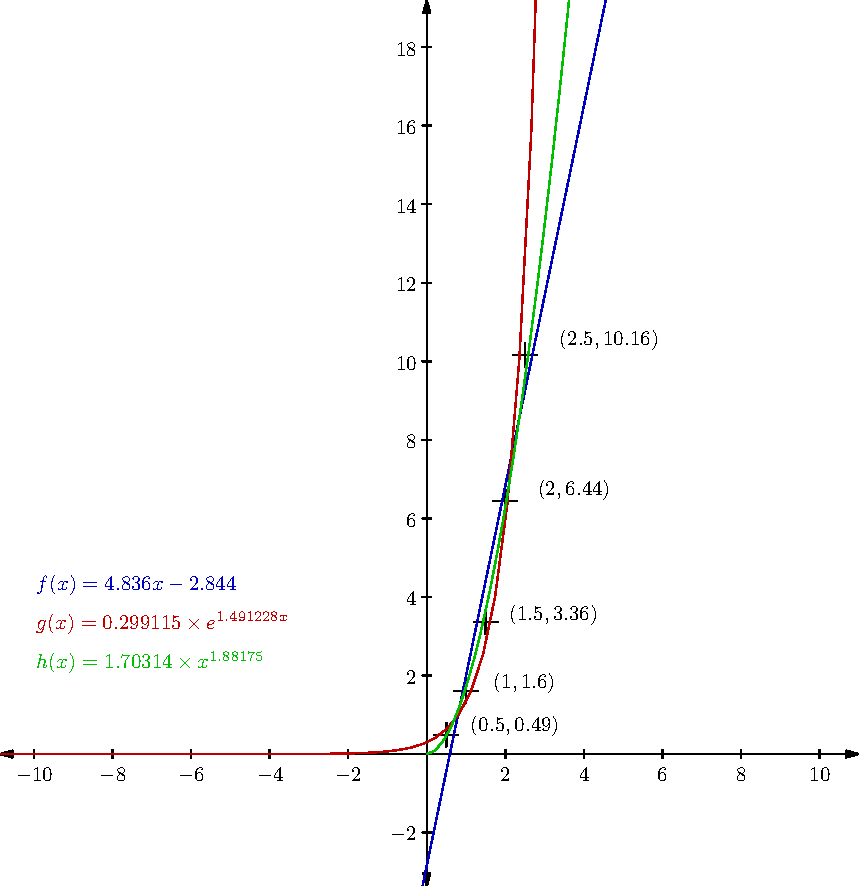
\includegraphics[scale=0.8]{graphiques/pdf_output/reglin.pdf}
	  \caption{Régression linéaire -- (Tableau \ref{approx_td3_ex6})}
	\end{figure}
      \newpage
      \subsection{Série d'Anscombe}
	\begin{table}[h]
	  \centering
	  \begin{tabular}{| c | c | c | c | c | c | c | c | c | c | c | c |}
	    \hline 
	    $x_{i}$ & $10$ & $8$ & $13$ & $9$ & $11$ & $14$ & $6$ & $4$ & $12$ & $7$ & $5$ \\ 
	    \hline 
	    $y^{(A)}_{i}$ & $8.04$ & $6.95$ & $7.58$ & $8.81$ & $8.33$ & $9.96$ & $7.24$ & $4.26$ & $10.84$ & $4.82$ & $5.68$ \\ 
	    \hline 
	  \end{tabular}
	  \caption{Série dûe à Anscombe}
	  \label{approx_tp2_ex1}
	\end{table}
	
	\begin{tabular}{l | l | l}
	\noindent \textbf{Régression linéaire : } & \noindent \textbf{Ajustement exponentiel} & \noindent \textbf{Ajustement ``puissance"} \\
	$P(x) = 0.500091x + 3.000091$ & $P(x) = 3.804664 \cdot e^{0.071377\cdot x}$ & $P(x) = 2.020991 \cdot x^{0.599390}$\\
	Erreur : $0.837405$ & Erreur : $0.933867$ & Erreur : $0.827968$ \\
	\end{tabular}
	\vspace{1cm}
	
	Note : Un ajustement de type ``puissance" permet d'obtenir une précision de $0.827968$, ce qui est très proche de celle obtenue ici. L'ajustement exponentiel est moins adapté.
	\begin{figure}[h]
	  \centering
	  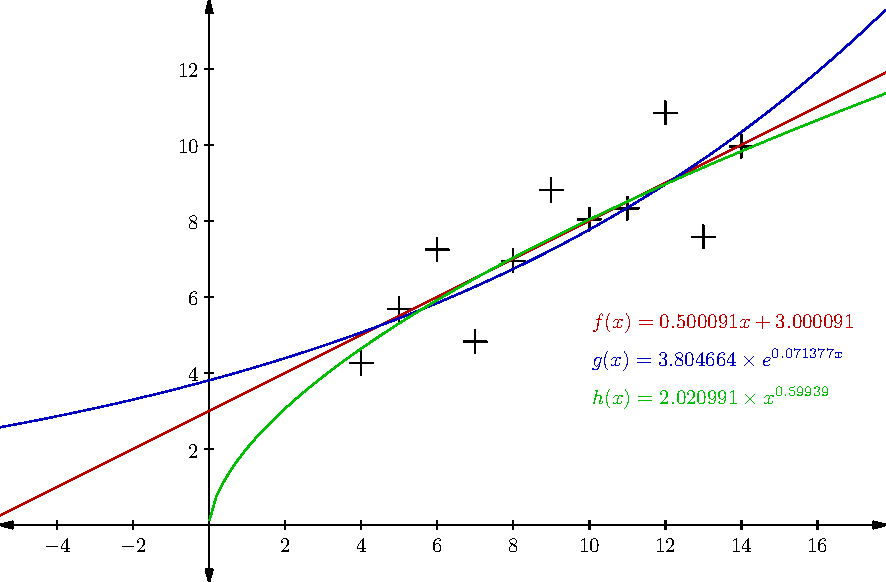
\includegraphics{graphiques/pdf_output/reglin_tp2_ex1.pdf}
	  \caption{Régression linéaire -- (Tableau \ref{approx_tp2_ex1})}
	\end{figure}
	\newpage
      \subsection{3 séries}
	\begin{table}[h]
	  \centering
	  \begin{tabular}{| c | c | c | c | c | c | c | c | c | c | c | c |}
	    \hline 
	    $x_{i}$ & $10$ & $8$ & $13$ & $9$ & $11$ & $14$ & $6$ & $4$ & $12$ & $7$ & $5$ \\ 
	    \hline 
	    $y^{(1)}_{i}$ & $9.14$ & $8.14$ & $8.74$ & $8.77$ & $9.26$ & $8.10$ & $6.13$ & $3.10$ & $9.13$ & $7.26$ & $4.74$ \\ %s1
	    \hline 
	    $y^{(2)}_{i}$ & $7.46$ & $6.77$ & $12.74$ & $7.11$ & $7.81$ & $8.84$ & $6.08$ & $5.39$ & $8.15$ & $6.42$ & $5.73$ \\ %s2
	    \hline 
	    $y^{(3)}_{i}$ & $6.58$ & $5.76$ & $7.71$ & $8.84$ & $8.47$ & $7.04$ & $5.25$ & $12.50$ & $5.56$ & $7.91$ & $6.89$ \\ %s3
	    \hline 
	    $y^{(A)}_{i}$ & $8.04$ & $6.95$ & $7.58$ & $8.81$ & $8.33$ & $9.96$ & $7.24$ & $4.26$ & $10.84$ & $4.82$ & $5.68$ \\ %anscombe
	    \hline 
	  \end{tabular}
	  \caption{3 séries $S^{(1)}$, $S^{(2)}$ et $S^{(3)}$ comparées à Anscombe}
	  \label{approx_tp2_ex2}
	\end{table}
	\begin{tabular}{l | l | l}
	  \noindent \underline{\textbf{Série 1 :}}  & \noindent\underline{\textbf{Série 2 :}} & \noindent\underline{\textbf{Série 3 :}} \\
	  \textbf{Régression linéaire : } & \textbf{Régression linéaire : } & \textbf{Régression linéaire : } \\
	  $P(x) = 3.000909 + 0.500000 \cdot x$ & $P(x) = 3.002455 + 0.499727 \cdot x$ & $P(x) = 9.231364 - 0.192273 \cdot x $\\
	  Erreur : $0.967934$ & Erreur : $0.715967$ & Erreur : $0.902727$ \\
	  & &\\
	  \textbf{Ajustement exponentiel : } & \textbf{Ajustement exponentiel : } & \textbf{Ajustement exponentiel : } \\
	  $P(x) = 3.417548 \cdot e^{0.082249 \cdot x}$ & $P(x) = 4.100273 \cdot e^{0.063981 \cdot x}$ & $P(x) = 8.564272 \cdot e^{-0.017989\cdot x}$\\
	  Erreur : $1.187786$ & Erreur : $0.590601$ & Erreur : $1.468203$\\
	  & & \\
	  \textbf{Ajustement ``puissance" : } & \textbf{Ajustement ``puissance" : } & \textbf{Ajustement ``puissance" : } \\
	  $P(x) = 1.453451 \cdot x^{0.749910}$ & $P(x) = 2.478570 \cdot x^{0.507328}$ & $P(x) = 10.959075\cdot x^{-0.192021}$ \\
	  Erreur : $0.950634$ & Erreur : $0.682932$ & Erreur : $1.463448$ \\
	  
	\end{tabular}
	\vspace{1cm}
	
	Pour la régression linéaire, il est important de remarquer que les deux premières séries donnent des équations de droites similaires et comparables à celle de la série d'Anscombe, tandis que la dernière varie complètement. On peut expliquer ceci par la présence de ``points isolés" ($(4,12.50)$ pour la série $S^{(3)}$) qui influent sur le calcul de l'équation. Ainsi on obtient des équations similaires pour des séries de points très différentes.\\ \\
	
	On notera aussi que la série $S^{(2)}$ possède un point isolé $(13,12.74)$, et que tous les autres points semblent appartenir à la même droite. Ce point a tendance à ``tirer" la droite vers le haut et donc à augmenter l'écart qui aurait pu être obtenu en l'absence de ce point.\\ \\
	
	Les ajustements de types exponentiel et ``puissance" donnent des écarts variables. Par exemple, il vaudra mieux approximer la série $S^{(1)}$ par puissance ou par régression, et la série $S^{(2)}$ avec un ajustement exponentiel. La série $S^{(3)}$ est composée d'un nuage de points, tout comme celle du test précédent (Anscombe), et les résultats montrent pour ces deux séries que des approximations par régression linéaire ou par ajustement ``puissance" sont plus appropriés que l'ajustement exponentiel.
	
	\newpage
	\begin{figure}[h!]
	  \centering
	  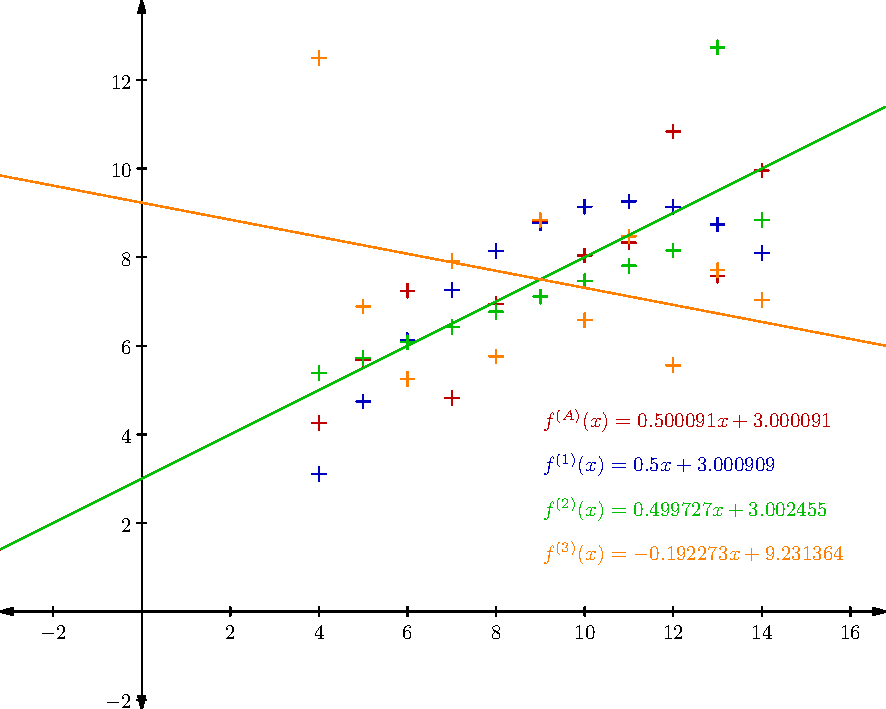
\includegraphics[scale=0.75]{graphiques/pdf_output/reglin_tp2_ex2_1.pdf}
	  \caption{Régression linéaire -- (Tableau \ref{approx_tp2_ex2})}
	\end{figure}

	\begin{figure}[h!]
	  \centering
	  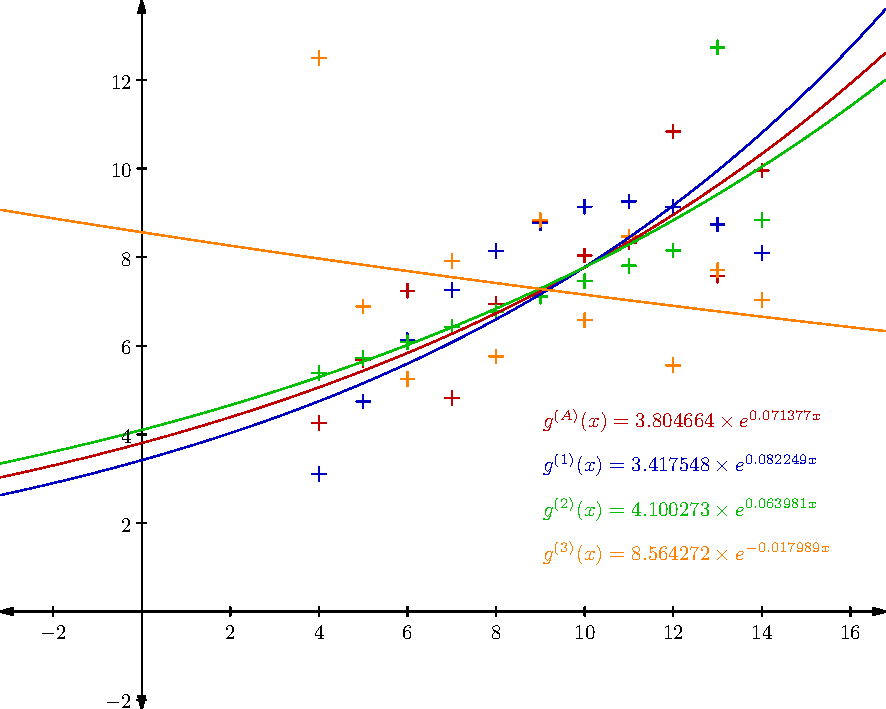
\includegraphics[scale=0.75]{graphiques/pdf_output/reglin_tp2_ex2_2.pdf}
	  \caption{Approximation par ajustement exponentiel -- (Tableau \ref{approx_tp2_ex2})}
	\end{figure}
	\newpage
	\begin{figure}[h!]
	  \centering
	  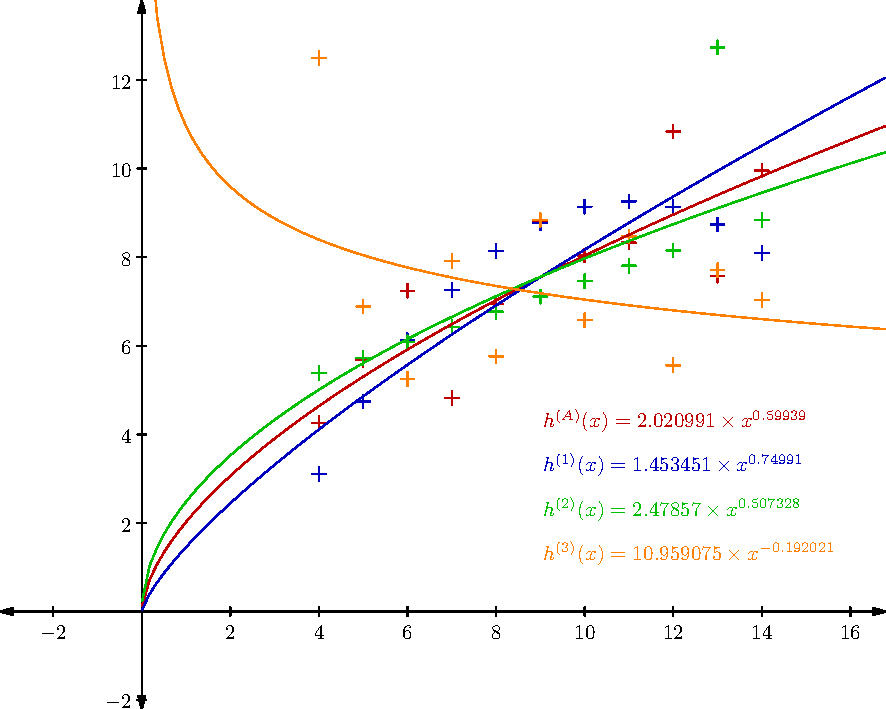
\includegraphics[scale=0.75]{graphiques/pdf_output/reglin_tp2_ex2_3.pdf}
	  \caption{Approximation par ajustement ``puissance" -- (Tableau \ref{approx_tp2_ex2})}
	\end{figure}
      \newpage
      \subsection{Dépenses mensuelles et revenus}
	\begin{table}[h]
% 	  \centering
	  \begin{tabular}{| c | c | c | c | c | c | c | c | c | c | c | c |}
	    \hline 
	    $x_{i}$ (R) & $752$ & $855$ & $871$ & $734$ & $610$ & $582$ & $921$ & $492$ & $569$ & $462$ & $907 $ \\ 
	    \hline 
	    $y_{i}$ (D) & $85$ & $83$ & $162$ & $79$ & $81$ & $83$ & $281$ & $81$ & $81$ & $80$ & $243 $ \\ 
	    \hline 
	  \end{tabular}
	  \newline
	  \begin{tabular}{| c | c | c | c | c | c | c | c | c | c | c |}
	    \hline 
	    $x_{i}$ (R) & $643$ & $862$ & $524$ & $679$ & $902$ & $918$ & $828$ & $875$ & $809$ & $894$ \\ 
	    \hline 
	    $y_{i}$ (D) & $84$ & $84$ & $82$ & $80$ & $226$ & $260$ & $82$ & $186$ & $77$ & $223$ \\ 
	    \hline 
	  \end{tabular}
	  \caption{Série non-triée}
	  \label{approx_tp2_ex3_depenses}
	\end{table}
	
	Comme pour l'interpolation, on peut trier les séries :
	
	\begin{table}[h]
	  \centering
	  \begin{tabular}{| c | c | c | c | c | c | c | c | c | c | c | c | c | c | c |}
	    \hline 
	    $x_{i}$ (R) & $752$ & $855$ & $828$ & $734$ & $809$ & $610$ & $582$ & $492$ & $569$ & $462$ & $643$ & $862$ & $524$ & $679$ \\ 
	    \hline 
	    $y_{i}$ (D) & $85$ & $83$ & $82$ & $79$ & $77$ & $81$ & $83$ & $81$ & $81$ & $80$ & $84$ & $84$ & $82$ & $80$ \\ 
	    \hline 
	  \end{tabular}
	  \caption{Série triée : Partie Basse}
	  \label{approx_tp2_ex3_depenses_bas}
	\end{table}
	\begin{table}[h]
	  \centering
	  \begin{tabular}{| c | c | c | c | c | c | c | c |}
	    \hline 
	    $x_{i}$ (R) & $902$ & $918$ & $871$ & $875$ & $921$ & $907$ & $894$ \\ 
	    \hline 
	    $y_{i}$ (D) & $226$ & $260$ & $162$ & $186$ & $281$ & $243$ & $223$ \\ 
	    \hline 
	  \end{tabular}
	  \caption{Série triée : Partie Haute}
	  \label{approx_tp2_ex3_depenses_haut}
	\end{table}
	
	\noindent\underline{\textbf{Valeurs non-triées :}} \\ \\
	\textbf{Régression Linéaire :}\\
	$P(x) = - 112.658491 + 0.324356\cdot x$\\
	Erreur : $43.378231$
	\newline
	\newline
	
	\noindent\underline{\textbf{Partie Basse :}} \\ \\
	\textbf{Régression Linéaire :}\\
	$P(x) = 80.112013 + 0.002173\cdot x$\\
	Erreur : $1.607015$
	\newline
	\newline
	
	\noindent\underline{\textbf{Partie Haute :}} \\ \\
	\textbf{Régression Linéaire :}\\
	$P(x) = -1632.996024 + 2.069334\cdot x$\\
	Erreur : $6.422749$
	
	\newpage
        \begin{figure}[h]
	  \centering
	  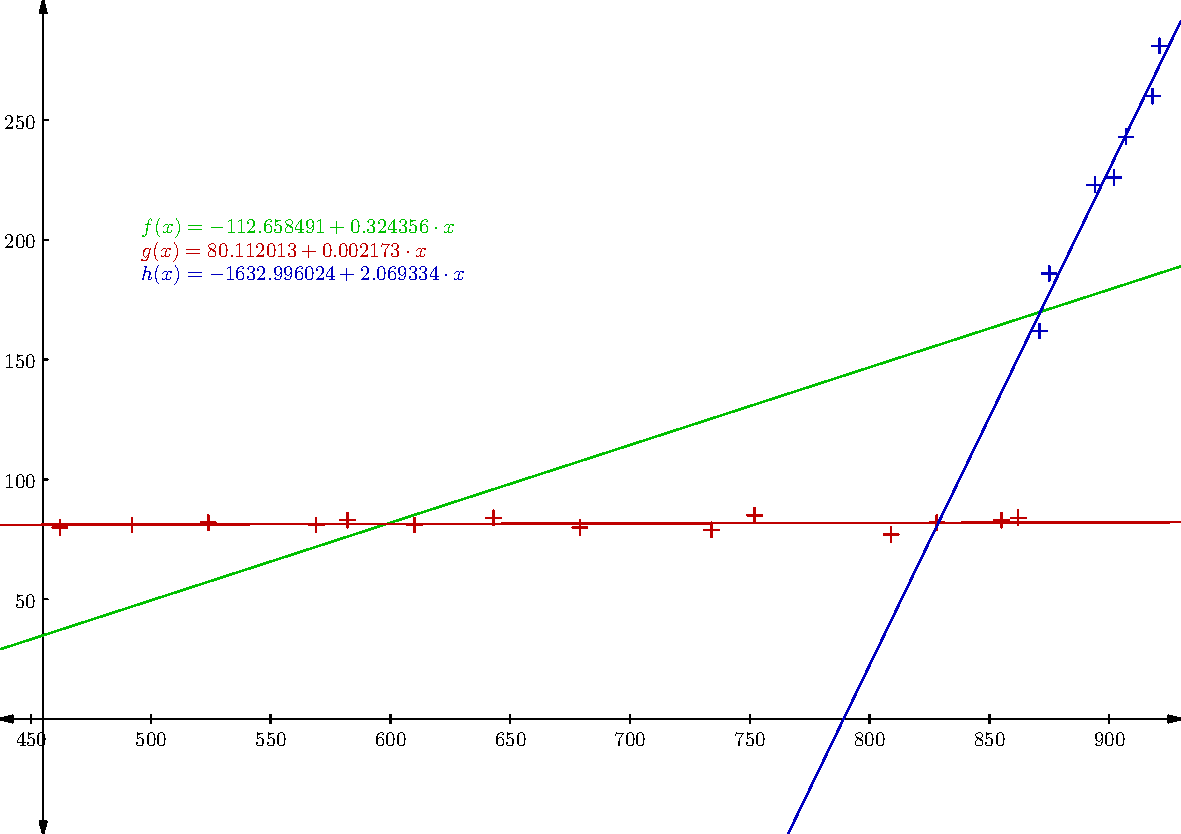
\includegraphics[scale=0.75]{graphiques/pdf_output/reglin_tp2_ex3.pdf}
	  \caption{Régression Linéaire (Tableaux \ref{approx_tp2_ex3_depenses} à \ref{approx_tp2_ex3_depenses_haut})}
        \end{figure}
      
      \newpage
      \subsection{Série chronologique avec accroissement exponentiel}
	\begin{table}[h]
	  \centering
	  \begin{tabular}{| c | c | c | c | c | c | c | c | c | c | c |}
	    \hline 
	    $x_{i}$ & $88$ & $89$ & $90$ & $91$ & $92$ & $93$ & $94$ & $95$ & $96$ & $97$ \\ 
	    \hline 
	    $y_{i}$ & $5.89$ & $6.77$ & $7.97$ & $9.11$ & $10.56$ & $12.27$ & $13.92$ & $15.72$ & $17.91$ & $22.13$ \\ 
	    \hline 
	  \end{tabular}
	  \caption{Série}
	  \label{approx_tp2_ex4}
	\end{table}
	
	\begin{figure}[h]
	  \centering
	  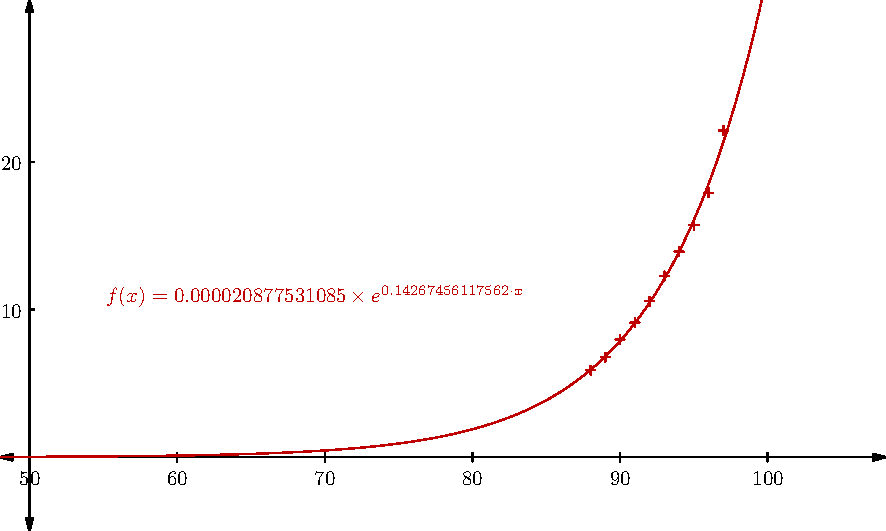
\includegraphics[scale=0.75]{graphiques/pdf_output/reglin_tp2_ex4.pdf}
	  \caption{Approximation par une fonction exponentielle (Tableau \ref{approx_tp2_ex4})}
        \end{figure}
      
      \newpage
      \subsection{Vérification de la loi de Pareto}
	\begin{table}[h]
	  \centering
	  \begin{tabular}{| c | c | c | c | c | c | c | c |}
	      \hline 
	      $x_{i}$ & $20$ & $30$ & $40$ & $50$ & $100$ & $300$ & $500$ \\ 
	      \hline 
	      $y_{i}$ & $352$ & $128$ & $62.3$ & $35.7$ & $6.3$ & $0.4$ & $0.1$ \\ 
	      \hline 
	  \end{tabular}
	  \caption{Relation entre revenu et nombre de personnes ayant un revenu supérieur}
	  \label{approx_tp2_ex5}
	\end{table}
	
	\begin{figure}[h]
	  \centering
	  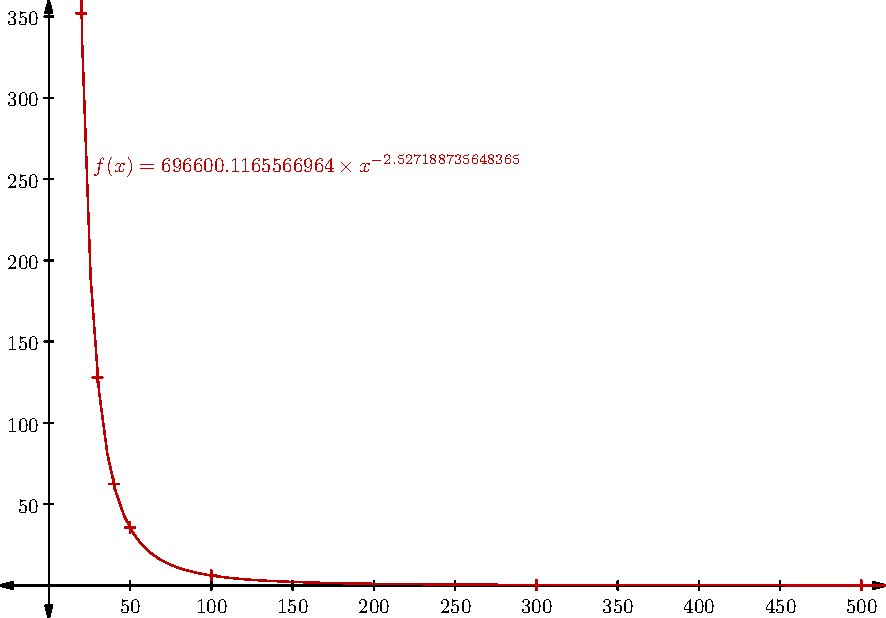
\includegraphics[scale=0.75]{graphiques/pdf_output/reglin_tp2_ex5.pdf}
	  \caption{Approximation par une fonction de type ``puissance" (Tableau \ref{approx_tp2_ex5})}
        \end{figure}
  \chapter{Conclusion}
  
  \chapter{Annexe}
    \section{Menu principal}
      \lstinputlisting[style=customc]{main.c}
    \section{Fonctions associées au calcul polynômial}
      \lstinputlisting[style=customc]{polynome.h}
      \lstinputlisting[style=customc, label=fonctionspolynome]{polynome.c}

\end{document}